\documentclass[journal,12pt,twocolumn]{IEEEtran}

\usepackage{setspace}
\usepackage{gensymb}
\singlespacing
\usepackage[cmex10]{amsmath}

\usepackage{amsthm}

\usepackage{mathrsfs}
\usepackage{txfonts}
\usepackage{stfloats}
\usepackage{bm}
\usepackage{cite}
\usepackage{cases}
\usepackage{subfig}

\usepackage{longtable}
\usepackage{multirow}

\usepackage{enumitem}
\usepackage{mathtools}
\usepackage{steinmetz}
\usepackage{tikz}
\usepackage{circuitikz}
\usepackage{verbatim}
\usepackage{tfrupee}
\usepackage[breaklinks=true]{hyperref}
\usepackage{graphicx}
\usepackage{tkz-euclide}

\usetikzlibrary{calc,math}
\usepackage{listings}
    \usepackage{color}                                            %%
    \usepackage{array}                                            %%
    \usepackage{longtable}                                        %%
    \usepackage{calc}                                             %%
    \usepackage{multirow}                                         %%
    \usepackage{hhline}                                           %%
    \usepackage{ifthen}                                           %%
    \usepackage{lscape}     
\usepackage{multicol}
\usepackage{chngcntr}

\DeclareMathOperator*{\Res}{Res}

\renewcommand\thesection{\arabic{section}}
\renewcommand\thesubsection{\thesection.\arabic{subsection}}
\renewcommand\thesubsubsection{\thesubsection.\arabic{subsubsection}}

\renewcommand\thesectiondis{\arabic{section}}
\renewcommand\thesubsectiondis{\thesectiondis.\arabic{subsection}}
\renewcommand\thesubsubsectiondis{\thesubsectiondis.\arabic{subsubsection}}


\hyphenation{op-tical net-works semi-conduc-tor}
\def\inputGnumericTable{}                                 %%

\lstset{
%language=C,
frame=single, 
breaklines=true,
columns=fullflexible
}
\begin{document}


\newtheorem{theorem}{Theorem}[section]
\newtheorem{problem}{Problem}
\newtheorem{proposition}{Proposition}[section]
\newtheorem{lemma}{Lemma}[section]
\newtheorem{corollary}[theorem]{Corollary}
\newtheorem{example}{Example}[section]
\newtheorem{definition}[problem]{Definition}

\newcommand{\BEQA}{\begin{eqnarray}}
\newcommand{\EEQA}{\end{eqnarray}}
\newcommand{\define}{\stackrel{\triangle}{=}}
\bibliographystyle{IEEEtran}
\raggedbottom
\setlength{\parindent}{0pt}
\providecommand{\mbf}{\mathbf}
\providecommand{\pr}[1]{\ensuremath{\Pr\left(#1\right)}}
\providecommand{\qfunc}[1]{\ensuremath{Q\left(#1\right)}}
\providecommand{\sbrak}[1]{\ensuremath{{}\left[#1\right]}}
\providecommand{\lsbrak}[1]{\ensuremath{{}\left[#1\right.}}
\providecommand{\rsbrak}[1]{\ensuremath{{}\left.#1\right]}}
\providecommand{\brak}[1]{\ensuremath{\left(#1\right)}}
\providecommand{\lbrak}[1]{\ensuremath{\left(#1\right.}}
\providecommand{\rbrak}[1]{\ensuremath{\left.#1\right)}}
\providecommand{\cbrak}[1]{\ensuremath{\left\{#1\right\}}}
\providecommand{\lcbrak}[1]{\ensuremath{\left\{#1\right.}}
\providecommand{\rcbrak}[1]{\ensuremath{\left.#1\right\}}}
\theoremstyle{remark}
\newtheorem{rem}{Remark}
\newcommand{\sgn}{\mathop{\mathrm{sgn}}}
\providecommand{\abs}[1]{\left\vert#1\right\vert}
\providecommand{\res}[1]{\Res\displaylimits_{#1}} 
\providecommand{\norm}[1]{\left\lVert#1\right\rVert}
%\providecommand{\norm}[1]{\lVert#1\rVert}
\providecommand{\mtx}[1]{\mathbf{#1}}
\providecommand{\mean}[1]{E\left[ #1 \right]}
\providecommand{\fourier}{\overset{\mathcal{F}}{ \rightleftharpoons}}
%\providecommand{\hilbert}{\overset{\mathcal{H}}{ \rightleftharpoons}}
\providecommand{\system}{\overset{\mathcal{H}}{ \longleftrightarrow}}
\providecommand{\ztrans}{\overset{\mathcal{Z}}{ \rightleftharpoons}}
	%\newcommand{\solution}[2]{\textbf{Solution:}{#1}}
\newcommand{\solution}{\noindent \textbf{Solution: }}
\newcommand{\cosec}{\,\text{cosec}\,}
\providecommand{\dec}[2]{\ensuremath{\overset{#1}{\underset{#2}{\gtrless}}}}
\newcommand{\myvec}[1]{\ensuremath{\begin{pmatrix}#1\end{pmatrix}}}
\newcommand{\mydet}[1]{\ensuremath{}}
\numberwithin{equation}{subsection}

\makeatletter
\@addtoreset{figure}{problem}
\makeatother
\let\StandardTheFigure\thefigure
\let\vec\mathbf

\renewcommand{\thefigure}{\theproblem}

\def\putbox#1#2#3{\makebox[0in][l]{\makebox[#1][l]{}\raisebox{\baselineskip}[0in][0in]{\raisebox{#2}[0in][0in]{#3}}}}
     \def\rightbox#1{\makebox[0in][r]{#1}}
     \def\centbox#1{\makebox[0in]{#1}}
     \def\topbox#1{\raisebox{-\baselineskip}[0in][0in]{#1}}
     \def\midbox#1{\raisebox{-0.5\baselineskip}[0in][0in]{#1}}
\vspace{3cm}
\title{Gate Assignment 4}
\author{Tanmay Goyal - AI20BTECH11021}
\maketitle
\newpage
\bigskip
\renewcommand{\thefigure}{\theenumi}
\renewcommand{\thetable}{\theenumi}

Download all latex codes from 
\begin{lstlisting}
https://github.com/tanmaygoyal258/EE3900-Linear-Systems-and-Signal-processing/blob/main/Quiz1/main.tex
\end{lstlisting}
\begin{lstlisting}
https://github.com/tanmaygoyal258/EE3900-Linear-Systems-and-Signal-processing/blob/main/Quiz1/code.py
\end{lstlisting}
\section{Problem}
(Oppenheim/2.33) Consider an LTI system with $\abs{H(e^{j\omega})} = 1$ and let $arg[H(e^{j\omega)}]$ be shown in the figure.  If the input is:
\begin{align}
    x[n] = \cos \brak{\frac{3\pi}{2}n + \frac{\pi}{4}}
\end{align}
find $y[n]$

\begin{figure}[!ht]
\centering
 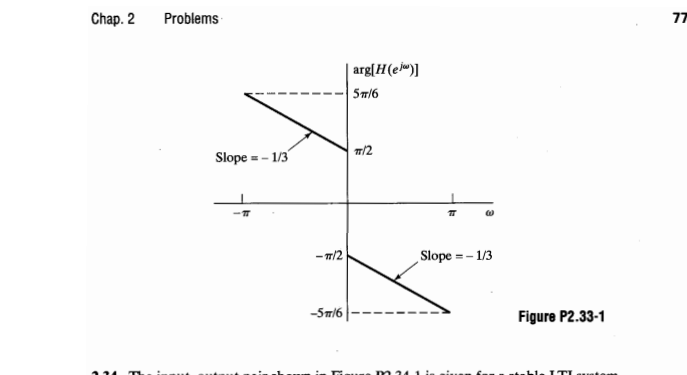
\includegraphics[width=\columnwidth]{Figure.png}
\end{figure}
\section{Solution}

\begin{lemma}\\
If 
\begin{align}
    x(t) \fourier X(j\omega)
\end{align}
then,
\begin{align}
    x^*(t) \fourier X^*(j\omega)
\end{align}
\begin{proof}
\begin{align}
    X(j\omega) = \int_{-\infty}^\infty x(t) e^{-j\omega t} \,dt\\
     X^*(j\omega) = \int_{-\infty}^\infty x^*(t) e^{j\omega t} \,dt\\
      X^*(-j\omega) = \int_{-\infty}^\infty x^*(t) e^{-j\omega t} \,dt
\end{align}
\end{proof}
\end{lemma}

\begin{lemma}
If $x(t)$ is real, then 
\begin{align}
    X(-j\omega) = X^*(j\omega)
\end{align}
\begin{proof}
\begin{align}
    X(j\omega) = \int_{-\infty}^\infty x(t) e^{-j\omega t} \,dt\\
     X^*(j\omega) = \int_{-\infty}^\infty x^*(t) e^{j\omega t} \,dt\\
      X^*(j\omega) = \int_{-\infty}^\infty x(t) e^{j\omega t} \,dt\\
       X(-j\omega) = X^*(j\omega)
\end{align}
using the fact that x is real and hence, $x^*(t) = x(t)$
\end{proof}
\end{lemma}

\begin{lemma}
If $x[n] = A \cos \brak{\omega_0 n + \phi}$, and if $h[n]$ is real, i.e $H(e^{-j\omega}) = H^*(e^{j\omega})$, then
\begin{align}
    y[n] = A \abs{H(e^{j\omega_0})}\cos \brak{\omega_0 n + \phi + arg(H(e^{j\omega_0})}
\end{align}
\label{ref}
\end{lemma}

Now, from the figure, we can write
\begin{align}
    arg[H(e^{j\omega})] = \begin{cases}
    -\frac{w}{3} + \frac{\pi}{2} &  -\pi<\omega<0\\
    -\frac{w}{3} -\frac{\pi}{2} &  0<\omega<\pi
    \end{cases}
    \label{arg}
\end{align}
Thus,
\begin{align}
    H(e^{j\omega}) = 
    \begin{cases}
    e^{j\brak{\frac{-w}{3} + \frac{\pi}{2}}} & -\pi < \omega < 0\\
    e^{j\brak{\frac{-w}{3} - \frac{\pi}{2}}} & 0<\omega<\pi
    \end{cases}\\
    H(e^{j\omega}) = 
    \begin{cases}
    je^{-\frac{j\omega}{3}} & -\pi < \omega < 0\\
    -je^{-\frac{j\omega}{3}} & 0<\omega<\pi
    \end{cases}\\
    \label{transfer}
\end{align}

Now, 
\begin{align}
    H(e^{-j\omega}) = 
    \begin{cases}
    je^{\frac{j\omega}{3}} & 0<\omega<\pi0\\
    -je^{\frac{j\omega}{3}} & -\pi < \omega < 0
    \end{cases}\\
    H^*(e^{j\omega}) = 
    \begin{cases}
    -je^{\frac{j\omega}{3}} & -\pi < \omega < 0\\
    je^{\frac{j\omega}{3}} & 0<\omega<\pi
    \end{cases}\\
    \implies H(e^{-j\omega}) = H^*(e^{j\omega})
\end{align}
Thus, using \eqref{ref}, we can say:
\begin{align}
    y[n] = 1\times \abs{H\brak{e^{\frac{j3\pi}{2}}}}\cos\brak{\frac{3\pi}{2}n + \frac{\pi}{4} + arg\sbrak{H\brak{e^{\frac{j3\pi}{2}}}}}\\
     = \cos\brak{\frac{3\pi}{2}n + \frac{\pi}{4} + arg\sbrak{H\brak{e^{\frac{j3\pi}{2}}}}}
     \end{align}

Now, to find $arg\sbrak{H\brak{e^{\frac{j3\pi}{2}}}}$, we have to realise that $H(e^{j\omega})$ is periodic with period $2\pi$, and thus from \eqref{arg}, we get:
\begin{align}
    arg\sbrak{H\brak{e^{\frac{j3\pi}{2}}}} = arg\sbrak{H\brak{e^{\frac{j3\pi}{2}} + j2n\pi}}\\
    arg\sbrak{H\brak{e^{\frac{j3\pi}{2}}}} = arg\sbrak{H\brak{e^{\frac{-j\pi}{2}}}}\\
    arg\sbrak{H\brak{e^{\frac{j3\pi}{2}}}} = \frac{2\pi}{3}
\end{align}
Thus, 
\begin{align}
    y[n] = \cos\brak{\frac{3\pi}{2}n + \frac{\pi}{4} + \frac{2\pi}{3}}\\
    y[n] = \cos\brak{\frac{3\pi}{2}n +  \frac{11\pi}{12}}
\end{align}
\begin{figure}[!ht]
\centering
 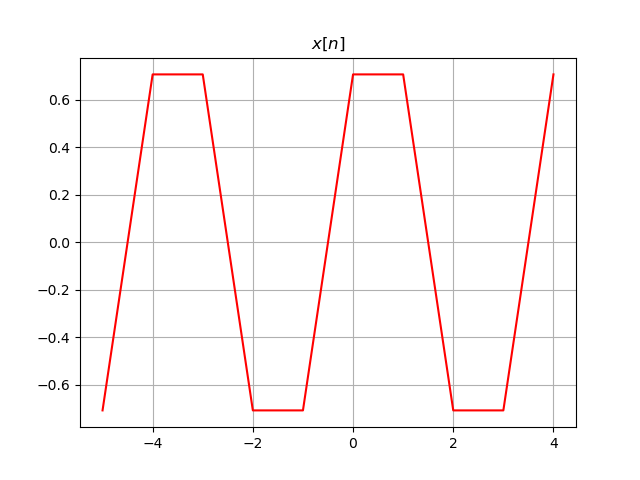
\includegraphics[width=\columnwidth]{Graphs/x_n.png}
 \caption{$x[n]$}
 \end{figure}
 \begin{figure}[!ht]
\centering
 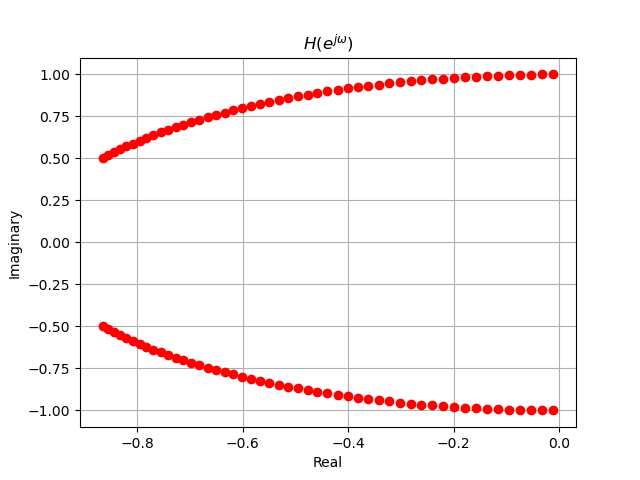
\includegraphics[width=\columnwidth]{Graphs/H.png}
 \caption{$H(e^{j\omega})$}
 \end{figure}
 \begin{figure}[!ht]
\centering
 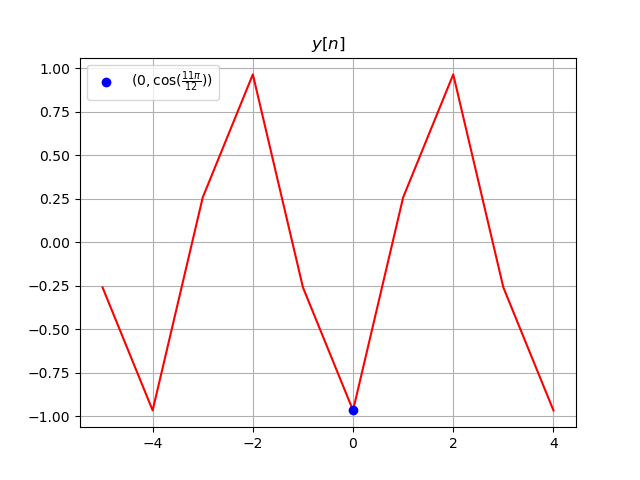
\includegraphics[width=\columnwidth]{Graphs/y.png}
 \caption{$y[n]$}
 \end{figure}
\end{document}